
%%%%%%% %%%%%%%%
\section*{General goal}

Perhaps we are presented with data: genome sequences plus other information
about a number of individuals that are usually random samples from some population(s),
and we want to learn about their shared history: 
estimate levels of relatedness between the samples;
infer their ancestral genome sequence(s);
or identify genomic locations subject to selection.
Or, perhaps we want to compute the levels of genetic diversity 
predicted under a certain population model.
In either case, we must understand the relationship between process parameters
(e.g.\ migration rates, selection coefficients)
and the observed genomic patterns of dissimilarity.

This discussion starts out from the unconvential direction
of treating the usual population genetic quantities as summary statistics
of the (unobserved) pedigree--with--recombination, the ``ancestral recombination graph'', or ARG.
Often, things like ``coalescent time'' are defined only in the context of mathematical models,
but can equally well be thought of as descriptive statistics,
whose expected values we can compute under certain models.
This seems to me at least conceptually useful when thinking about such quantities
as estimated from real data, where assumptions such as random mating are rarely met.

Some other discussions that take this point of view to at least some degree are:
\citet{mcvean2002linkage}, OTHERS.
% The textbook ``Tree Thinking'' XXX ALSO XXX ?
Other good references for coalescent theory are
\citet{hudson1990gene} (a nice article-length review), 
and the books
\citet{wakeley2005coalescent} (fairly gentle)
and \citet{ewens2004mathematical} (fairly mathematical, and covers more general population genetics).


%%%%%%% %%%%%%%%
\section{Recombination, segregation, and mutation}

First, an outline of how we model diploid reproduction, 
i.e.\ how the autosomal genome of an offspring gets assembled from those of the parents.
There are exceptions (of course), but mostly,
each organism has two copies of each autosomal chromosome, 
one from mom and one from dad.
Offspring are the union of two gametes (an egg and a spermatid),
and each gamete is produced by a single diploid cell:
\begin{itemize}
    \item duplicating each chromosome (by mitosis)
    \item recombining the homlogous copies
    \item segregating these copies among four daughter cells.
\end{itemize}
Sometimes all four daughter cells become gametes;
sometimes (e.g.\ female meiosis in mammals) only one will.


\paragraph{Recombination} is complicated, varies along the genome, and is affected by genomic factors and motifs.
To make it tractable, we assume that recombination breakpoints occur as a Poisson point process 
with constant mean of 2 breakpoints per unit of length,
and that each breakpoint is a crossing over between a randomly chosen maternal and a randomly chosen paternal chromosome.
This produces an average of 1 crossover per chromosome per unit length, 
i.e.\ we are measuring length in genetic map length (Morgans).


\paragraph{Mutation}
% We wouldn't have got far without ``descent \emph{with modification}'' -- and, from thence comes our data -- so we need mutation, also.
In a major concession to mathematical convenience, we'll simply model mutation as another Poisson point process --
suppose that each gamete differs from its progenitor chromosome at the points of an Poisson point process.
This is the ``infinite sites model'', assuming that mutation cannot hit at the same location twice.
Usually we assume the point process of mutations has mean rate $\mu$ per unit of map length,
but in reality this rate varies along the genome.

\paragraph{Segregation}
Once four gametes are produced, it remains to be decided which of the four produce the offspring.
We assume that one is chosen uniformly at random,
independently of the result of recombination.
(Again, there are exceptions.)


%%%%%%% %%%%%%%%
\section{The pedigree, with recombination}

The \emph{pedigree} of a set of individuals is a graph 
describing all parent-offspring relationships between these
and some set of their ancestors.
The \emph{population pedigree} describes all such relationships
between all individuals living and possibly dead.
This records mate choice,
but omits the important information of recombination and segregation,
i.e.\ which parts of each chromosome derive from which of the parents' two homologous copies.
Adding this information to the pedigree obtains what is known as the \emph{ancestral recombination graph}, or ARG.
There are a number of ways to formalize this notion;
see \citep{griffiths1997ancestral,hudson1990gene} for discussions.
One way simply notes that the relatedness structure at any particular locus
is a treelike subset of the pedigree,
and that the collection of these trees -- one for each base in the genome, say --
is sufficient to reconstruct the entire history of inheritance, recombination and segregation.
Alternatively, one can annotate each link in the pedigree with a labeling of the genome by $\{m,p\}$,
denoting which segments of the parent's maternal and paternal chromosomal copies were passed down along that link.
See figure \ref{fig:pedigree_ibd} for a partial depiction.

\begin{figure}[ht!]
  \begin{center}
    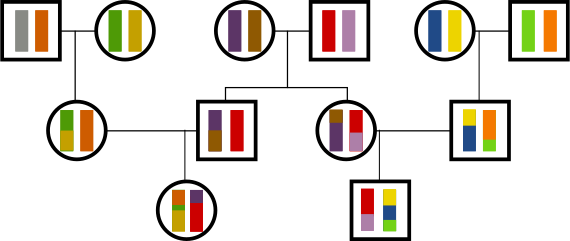
\includegraphics[width=3.5in]{pedigree-ibd-recombination}
  \end{center}
  \caption{
  A small pedigree relating two cousins to their six grandparents,
  with the extra information of recombination and segregation on one chromosome
  encoded by a coloring: each chromosome is composed
  of a patchwork of the grandparental chromosomes.
  XXX make additional figure showing marginal gene trees XXX
  \label{fig:pedigree_ibd}
  }
\end{figure}

%%%%%%% %%%%%%%%
\subsection{Coalescence times and gene trees}

Perhaps the simplest thing we can obtain from the full ancestral recombination graph 
is the typical degree of relatedness of pairs of individuals.
More concretely, we might ask for the empirical distribution
of pairwise times back to the most recent common ancestor
across all pairs of chromosomes and all loci:
the distribution of $\tau_T$, if $\tau_T$ is the length of a randomly chosen one of these paths.

A more precise way of formulating this is as follows:
pick two random chromosomes and a random locus;
follow the lineages of the two chromosomes at that locus up through the pedigree
until their common ancestor;
one-half the number of meioses encountered is $\tau_T$.
Since these two lineages will henceforth move together through if followed further back through the pedigree,
$\tau_T$ is known as the ``coalescence time'' of the two lineages.

In this way, the phrase ``coalescence time'' is shorthand
for ``number of generations back to the most recent common ancestor'',
taken as a random quantity across random samples of sets of chromosomes and/or loci.
In this formulation, it is the empirical distribution of lengths of a certain set of paths 
to common ancestors through the pedigree.

The path back through the pedigree along which these two chromosomes have inherited that particular locus
is a very simple tree, with two leaves (at the samples) and a root at their most recent common ancestor;
the height of that tree is the coalescence time.
More generally, the ancestral recombination graph encodes the marginal tree along which, 
at each locus, any set of sampled individuals have inherited at that locus.
These are called ``gene trees''.
Each gene tree follows a path through the links of the pedigree,
and if due to recombination during one of the meioses, 
loci $x$ and $y$ are inherited from different parental chromosomes,
the marginal gene trees at $x$ and $y$ will differ.


%%%%%%% %%%%%%%%%
\subsection{Formalities}

Now, a formal definition for the so far obvious-yet-vague ``ancestral recombination graph''.
This records all relationships between both chromsomes of all individuals that ever lived in the population:
so, let $\chrom_t$ denote those chromosomes that were alive at time $t$,
and let $\chrom = \bigcup_t \chrom_t$ denote all chromosomes in our universe,
These are furthermore grouped together into individuals:
$\indiv_t$ is a partition of $\chrom_t$ into pairs, and likewise $\indiv$ is a partition of $\chrom$ into pairs.
The relationships occur if two chromosomes in a diploid cell undergo recombination and meiosis,
producing one chromosome for an offspring.
So, if $(c_m,c_p)$ is a pair of chromosomes in $\indiv_t$,
and they recombine at locations $r=(r_1,r_2,\ldots,r_k)$
to produce chromsome $c$,
then we say that the meiosis $(c,c_m,c_p,r)$ has occurred.
As a matter of convention, say that $c$ has inherited from $c_m$ 
on odd intervals $[0,r_1)$, $[r_2,r_3)$, etcetera,
and has inherited from $c_p$ from the remaining intervals,
and that $0 \le r_1 < r_2 < \cdots < r_k = G$, where $G$ is the length of the chromosome.
Let $\meioses_t$ be the meioses occurring at $t$,
and $\meioses = \bigcup_t \meioses_t$.
To reiterate, if $(c,c_m,c_p,r) \in \meioses_t$, then
$c$ must be in an individual birthed at $t$ from living parents; 
i.e.\ $c \in \chrom_t$ but $c \notin \chrom_s$ for any $s<t$;
and $(c_m,c_p) \in indiv_t$.

Note that it is natural to identify each chromosome with the meiosis that produced it.

All the information required to construct the population pedigree
(who was whose parents) is contained in $\meioses$;
also, the gene tree at each location along the genome.

For instance, let $T_x$ be the gene tree for a set of samples at position $x$ along the genome.
This is the minimal acyclical graph (a tree) whose nodes are chromosomes (or, equivalently, meioses), 
that contains the sampled chromosomes,
and if a chromosome $c$ is in $T_x$, then so is the parent of $c$ at which $c$ has inherited at $x$.
These trees change whenever a breakpoint is encountered in any of the constituent meioses:
Formally, define $R(c)$ to be the set of recombination breakpoints of the meiosis that created $c$;
then the next point to the right of $x$ at which the tree changes is:
\begin{align}
  \inf\{ y > x \st T_y \neq T_x \} = \inf\{ z \st z > x \; \text{and} \; z \in \bigcup_{c\in T_x} R(c) \} .
\end{align}


This notation, so far, describes the facts:
actual relationships that have already occurred in a population;
many of which may be unobservable.
To make inferences, we will need to put models of certain of these processes:
on mutation, recombination, mate choice, and/or offspring number.


%%%%%%% %%%%%%%%%%%%
\section{Conventions and definitions}

\paragraph{Generations}
  When two chromosomes share a common ancestor, we like to say that that ancestor lived some number of ``generations'' in the past.
  For most organisms, the notion of a generation is statistical, rather than a fixed quantity.
  What we actually care about is the number of meioses separating the two chromosomes --
  so, we hereby define the length of a path through the pedigree in generations as one-half the number of meioses.
  In fact, in the presence of inbreeding, it is possible for two chromosomes to have inherited different genomic regions
  from the same ancestor along different paths through the pedigree, which may have different lengths!

\paragraph{Mutation process}
  We will mostly work in the \emph{infinite alleles} model of mutation
  (which assumes that any mutation produces a unique allele)
  and that mutation rates are homogeneous along the genome.
  This is clearly not correct, but a very good approximation over the right scales.


\paragraph{Discrete or continuous rates}
  Here we define $\mu_d$ to be the (``discrete'') mutation rate per generation per base 
  -- the probability that a given base differs from the homologous base in the parent it was inherited from.
  We will sometimes find it convenient to use $\mu = -\log(1-\mu_d)$,
  so that the probability of no mutation across $2t$ meioses is $(1-\mu_d)^{2t} = \exp(-2 t \mu )$.

